\section{PC} \label{sec:PC}

\begin{figure}[h!]
\centering
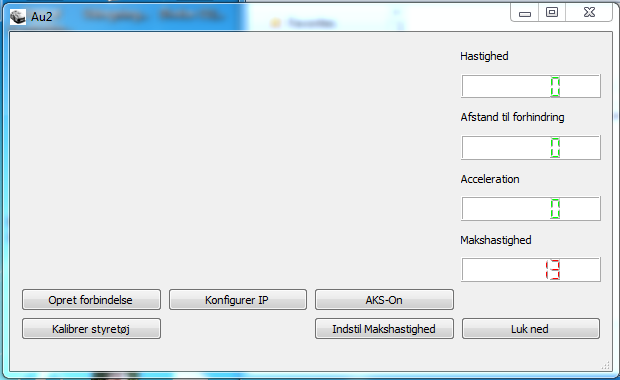
\includegraphics[width=\textwidth* 3/4]{../fig/billeder/gui_start.png}
\caption{GUI hovedvindue}
\label{fig:GUI_hovedvindue}
\end{figure}

\subsection{Sekvensdiagrammer}

I denne sektion beskrives sekvensdiagrammer over usecasene for GUI'en. Der er valgt at lave i alt 4 scenarier af UC1 hvor 3 af dem inkluderer fejl. Dette er gjort for at gøre det mere overskueligt, da et sekvensdiagram med en masse undtagelser hurtigt bliver forvirrende.På figur
\ref{fig:cd_uc1_succes_gui} ses sekvensdiagrammet over UC1 scenarie: succes.

\subsubsection{UC1 Succes}

\begin{figure}[ht]
\centering
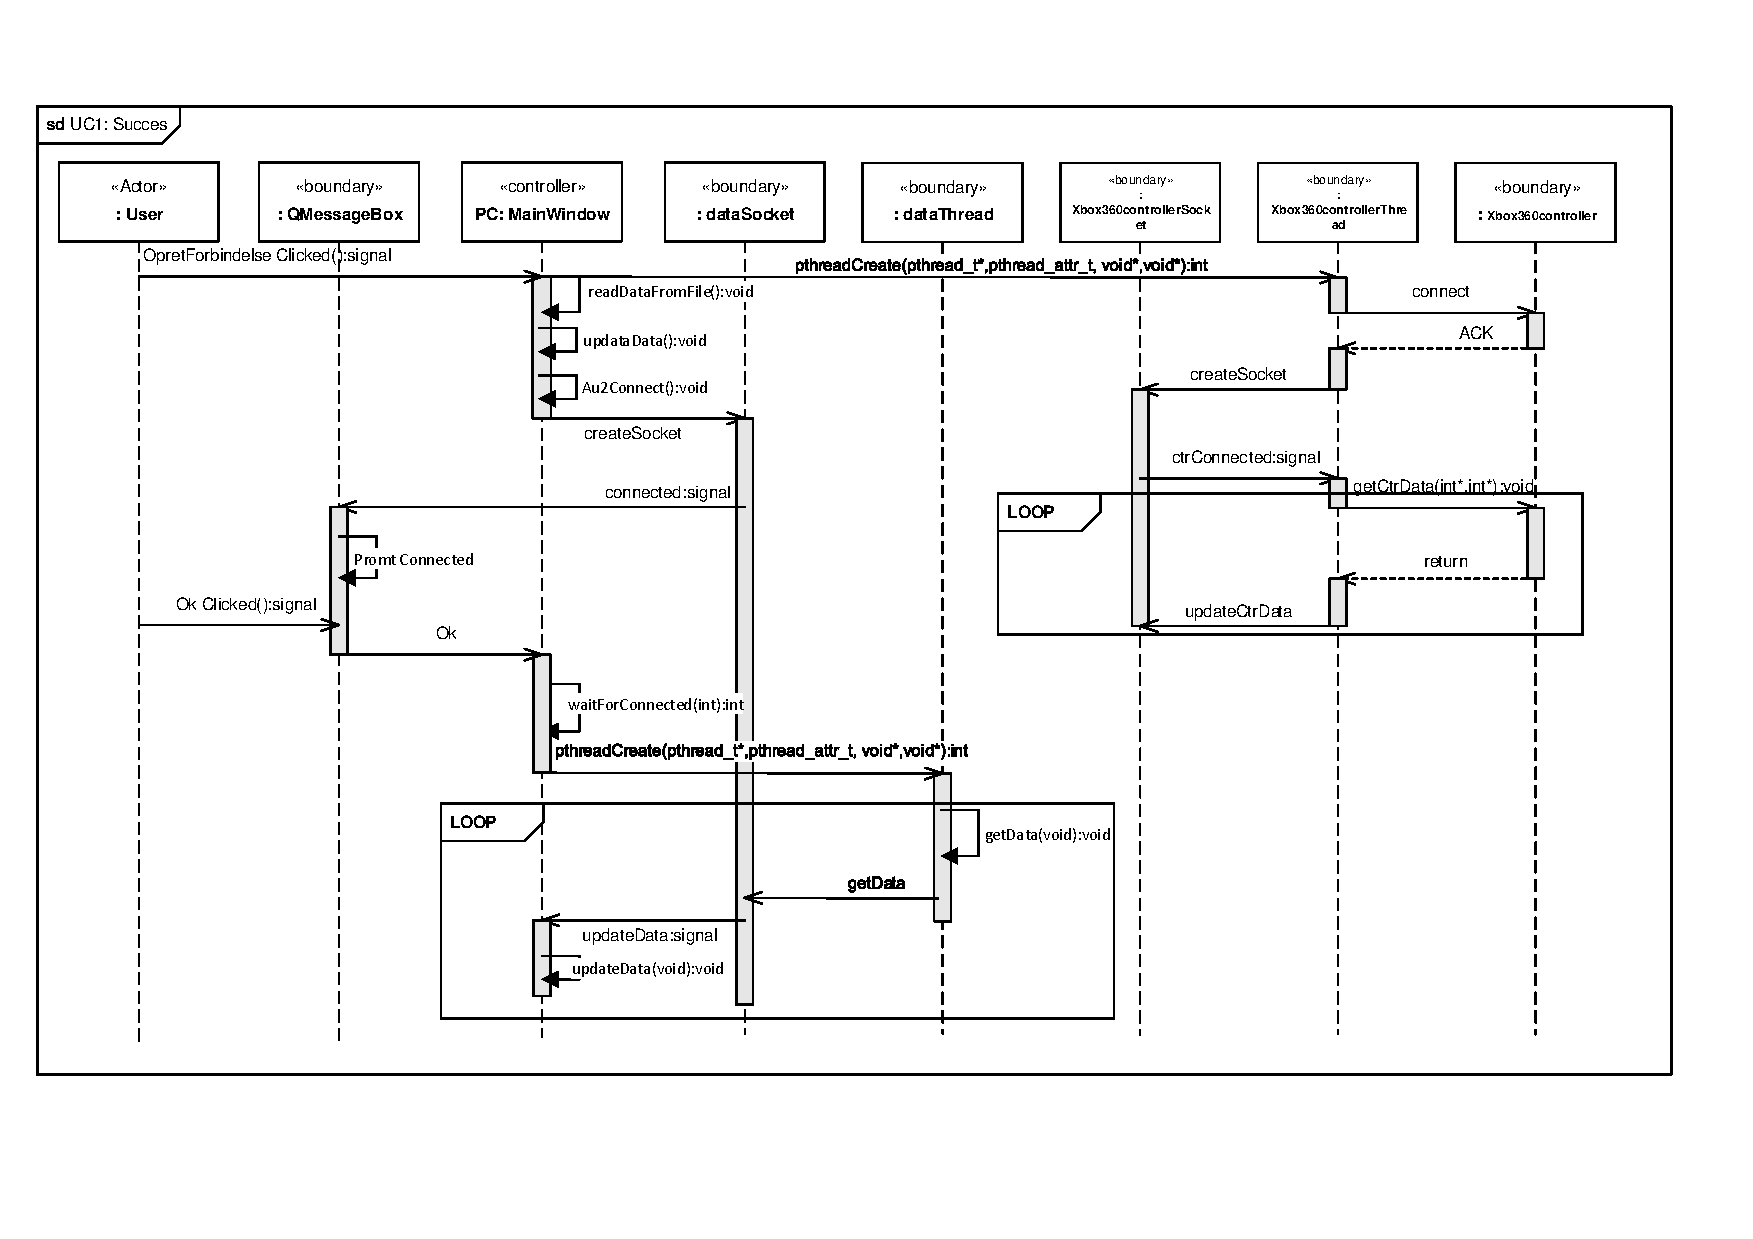
\includegraphics[width=\textwidth* 1,]{../fig/diagrammer/pc/sd_uc1_succes.pdf}
\caption{Sekvensdiagram over UC1 senarie:succes}
\label{fig:cd_uc1_succes_gui}
\end{figure}

Når usecasen startes klikker brugeren på \texttt{''Opret forbindelse''} på GUI'en.
Herefter vil \texttt{MainWindow} starte Xbox360ControllerThread, som vil oprette en socketforbindelse mellem bilen og PC til at sende controllerdata.\linebreak[2]
Efterfølgende vil \texttt{MainWindow} indlæse data, som blev gemt i logfilen sidste gang programmet lukkede ned og derefter opdatere vinduet. \linebreak[2]
Derefter vil \texttt{MainWindow} oprette en socket mere til at sende og modtage data fra og til bilen. \linebreak[2]
Når socketforbindelsen er oprettet vil \texttt{dataSocket} sende et signal til \texttt{MainWindow}, som derved vil promte brugeren at forbindelsen er oprettet. 
Se figur \ref{fig:GUI_uc1_success}. \linebreak[2]
Når brugeren lukker vinduet ved at klikke på \texttt{''Ok''} venter \texttt{MainWindow} på at der er forbindelse for at derefter oprette \texttt{dataThread} som efterfølgende vil stå for at opdatere vinduet med hastig, afstand, acceleration osv.  \linebreak[2]
Når brugeren trykker på ''Ok'' sættes en variabel til 1. \linebreak[2]
Hvis forbindelsen senere mistes sættes denne variabel til 0, således \texttt{dataThread} ikke skriver til en socketforbindelse som ikke længere er aktiv. 
Ventetiden er for at sikre at signalet kommer inden for en given tid.  \linebreak[2]
Defor: Kommer signalet om at forbindelsen ikke er oprettet inden for en given tid, vil programmet lave en fejl som det ses i figur \ref{fig:GUI_uc1_error_1}. \linebreak[2]
Når \texttt{dataThread} har opdateret dataen, vil den give et signal til \texttt{MainWindow} om at der skal hentes nye data fra bilen. \linebreak[2]
Det er derfor \texttt{MainWindow} som henter og sender data, men \texttt{dataThread} som opdatere selve dataen på GUI'en. \linebreak[2]
Dette skyldes at \texttt{QTcpsocket} ikke kan køres i en separat tråd som det gøres med \texttt{Xbox360ControllerThread} hvis der skal gives signaler. \linebreak[2]
Der sker derfor en fejl i programmet når Xbox360 controlleren er forbundet og TCP forbindelsen mistes. \linebreak[2]
Der har desværre ikke været tid til at finde en løsning på dette problem.  


\begin{figure}[ht!]
\centering
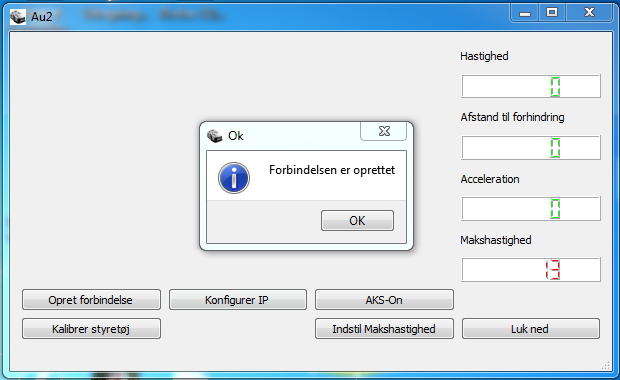
\includegraphics[width=\textwidth* 3/4]{../fig/billeder/gui_uc1_success.png}
\caption{GUI UC1 succes}
\label{fig:GUI_uc1_success}
\end{figure}

\clearpage

%=============== UC1 Error 1 =============
\subsubsection{UC1 Error 1: Forbindelse kunne ikke oprettes}
I denne sektion beskrives fejlen, at der ikke kan oprettes forbindelse til bilen når brugeren trykker på \texttt{''Opret forbindelse''}. Funktionen \texttt{waitForConnected} venter i maks et sekund, er der ikke oprettet forbindelse derefter promtes brugeren med at forbindelsen ikke kunne oprettes. Se sekvensdiagrammet i figur \ref{fig:cd_uc1_error_1} og advarselsskiltet i figur \ref{fig:GUI_uc1_error_1}

\begin{figure}[H]
\centering
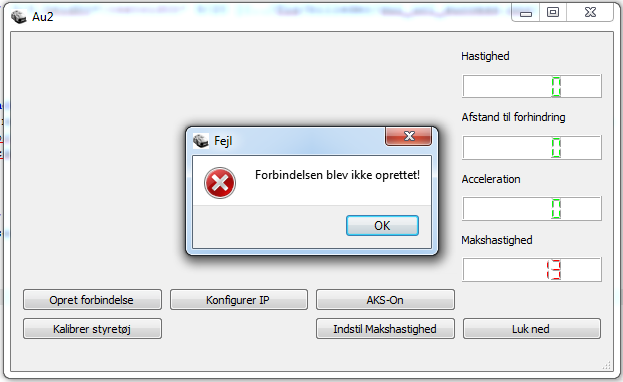
\includegraphics[width=\textwidth* 3/4]{../fig/billeder/gui_uc1_error_1.png}
\caption{GUI UC1 Error 1}
\label{fig:GUI_uc1_error_1}
\end{figure}

\begin{landscape}
\begin{figure}[H]
\centering
\includegraphics[width=\linewidth]{../fig/diagrammer/pc/sd_uc1_Error_1.pdf}
\caption{Sekvensdiagram over UC1 senarie:Error 1}
\label{fig:cd_uc1_error_1}
\end{figure}
\end{landscape}

\clearpage
%=============== UC1 Error 2 =============
\subsubsection{UC1 Error 2: Controller er ikke forbundet}
I denne sektion beskrives fejlen, at Xbox360-controlleren ikke er forbundet til PC'en. \linebreak[3] 
PC softwaren vil spørge om controlleren er tilsluttet når \texttt{Xbox360controllerThread} oprettes. 
Hvis ikke, vises fejlen i figur \ref{fig:GUI_uc1_error_2}. 
Se sekvensdiagrammet i figur \ref{fig:cd_uc1_error_2}.

\begin{figure}[h!]
\centering
\includegraphics[width=\textwidth* 1]{../fig/diagrammer/pc/sd_uc1_Error_2.pdf}
\caption{Sekvensdiagram over UC1 senarie:Error 2}
\label{fig:cd_uc1_error_2}
\end{figure}

\begin{figure}[h!]
\centering
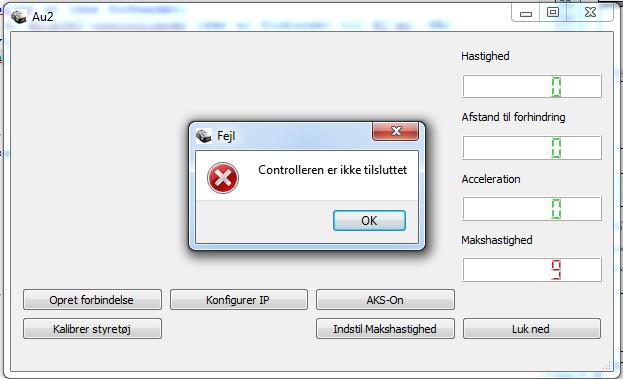
\includegraphics[width=\textwidth* 6/9]{../fig/billeder/gui_uc1_error_2.png}
\caption{GUI UC1 Error 2}
\label{fig:GUI_uc1_error_2}
\end{figure}

\clearpage

%=============== UC1 Error 3 =============
\subsubsection{UC1 Error 3: Forbindelsen bliver afbrudt}
I denne sektion beskrives fejlen, at forbindelsen mellem bil og PC pludselig bliver afbrudt. Dette sker ved at \texttt{dataSocket} giver signal til \texttt{MainWindow} om at forbindelsen er afbrudt, som herefter giver besked til brugeren. Herefter stopper \texttt{dataSocket} med at opdatere data. Er controlleren forbundet og bliver denne forbindelse også afbrudt crasher programmet desværre. Denne fejl er beskrevet tidligere. Se sekvensdiagrammet i figur \ref{fig:cd_uc1_error_3} og advarselsskiltet i figur \ref{fig:GUI_uc1_error_3} 

\begin{figure}[H]
\centering
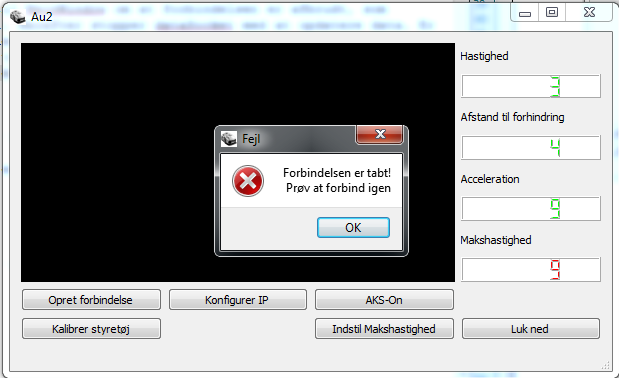
\includegraphics[width=\textwidth* 3/4]{../fig/billeder/gui_uc1_error_3.png}
\caption{GUI UC1 Error 3}
\label{fig:GUI_uc1_error_3}
\end{figure}
\vfill
\clearpage

\begin{landscape}
\begin{figure}
\centering
\includegraphics[width=\linewidth]{../fig/diagrammer/pc/sd_uc1_Error_3.pdf}
\caption{Sekvensdiagram over UC1 senarie:Error 3}
\label{fig:cd_uc1_error_3}
\end{figure}
\vfill
\end{landscape}

\clearpage

%=============== UC8 Konf IP =============
\subsubsection{UC8: Konfigurer IP-adresse}
For at aktivere usecase 8 klikker bruger på \texttt{''Konfigurer IP''}. Herefter åbner \texttt{MainWindow} en inputdialog som bruger indtaster IP-adressen i og efterfølgende trykker \texttt{''Ok''}. Se sekvensdiagrammet i figur \ref{fig:cd_uc8} og indputdialogen i figur \ref{fig:GUI_uc8} 

\begin{figure}[H]
\centering
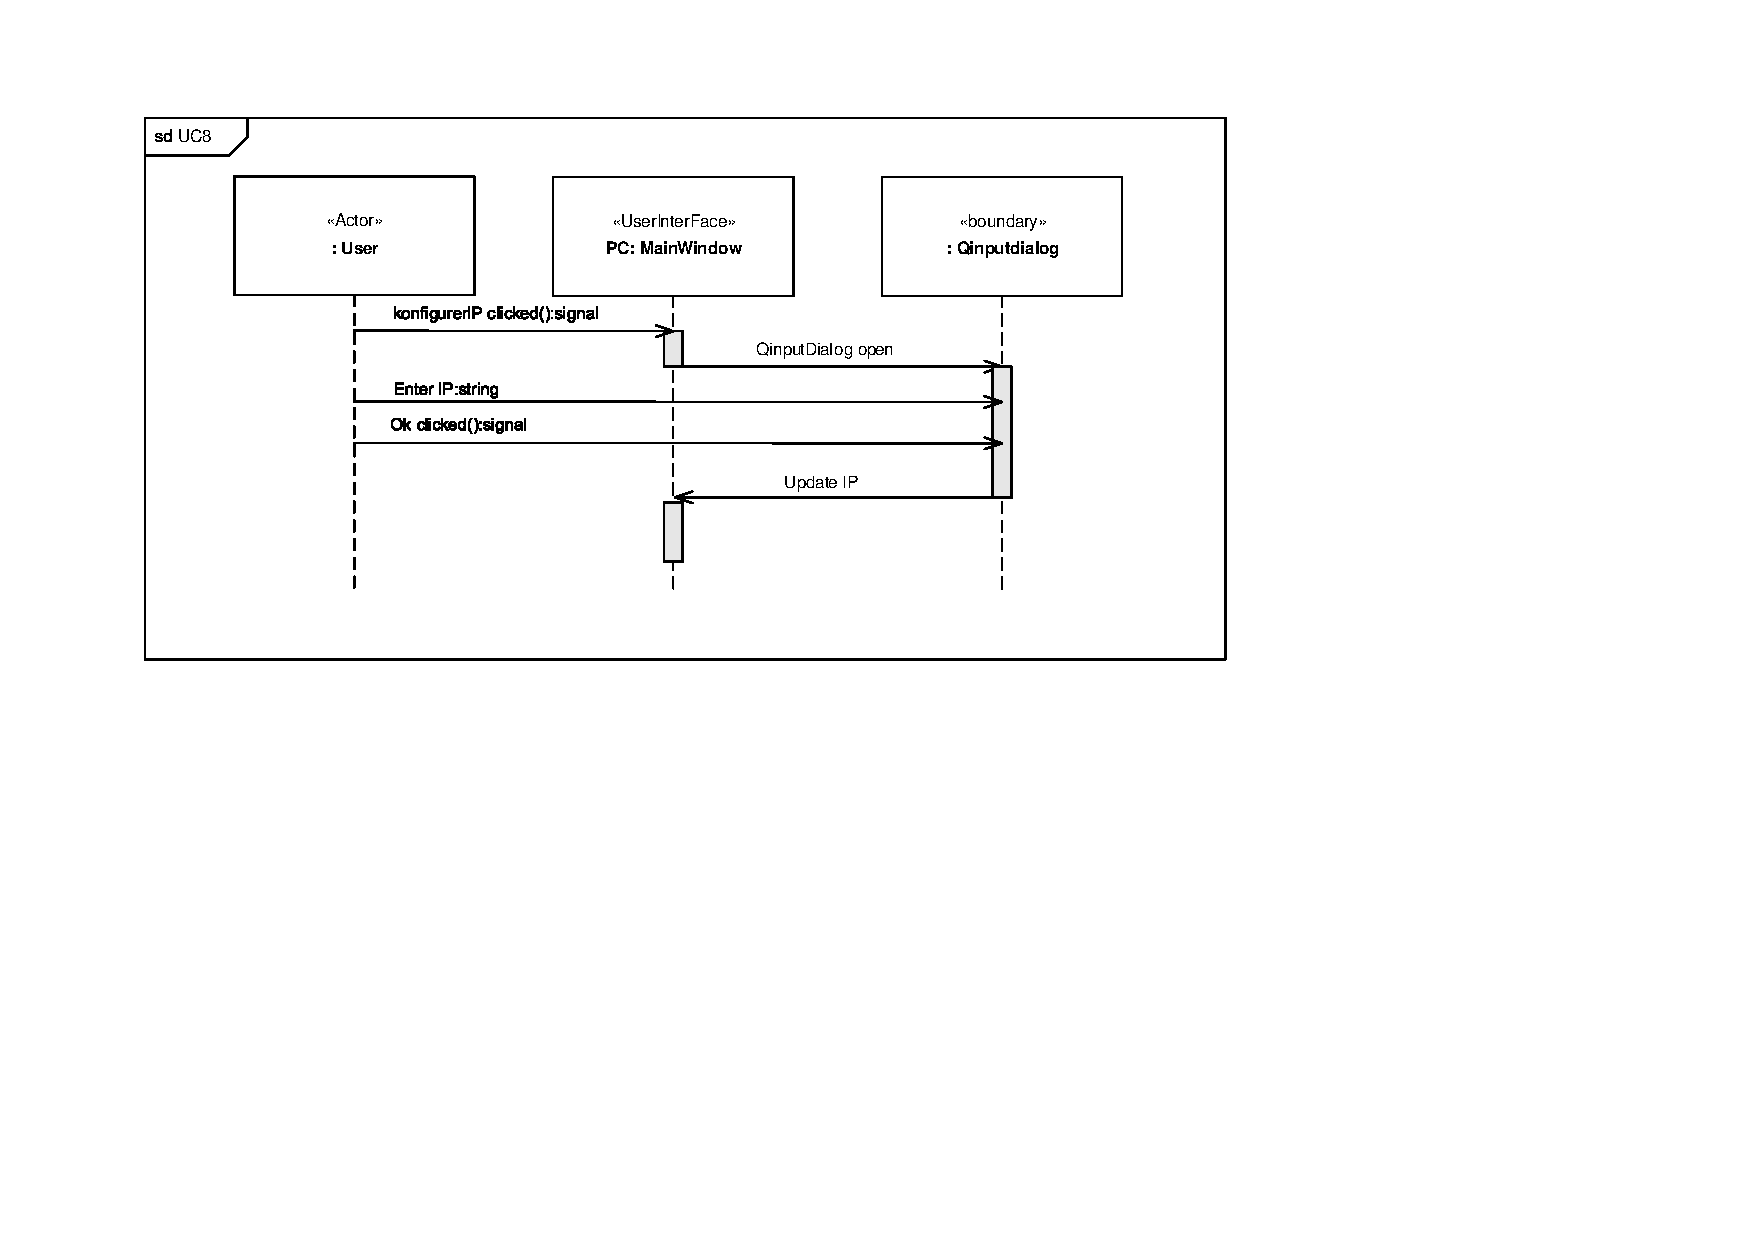
\includegraphics[width=\textwidth* 2/3,height=\textwidth* 4/10 ]{../fig/diagrammer/pc/sd_uc8.pdf}
\caption{Sekvensdiagram over UC8}
\label{fig:cd_uc8}
\end{figure}

\begin{figure}[H]
\centering
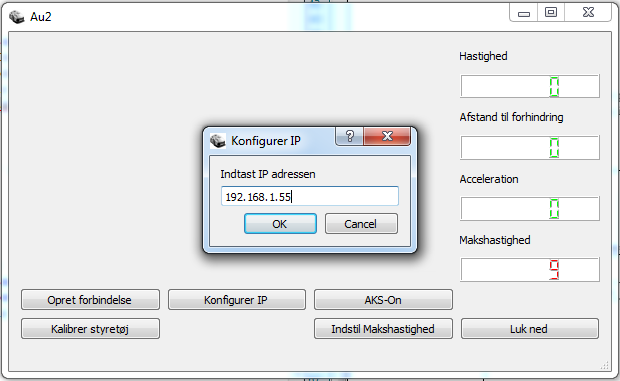
\includegraphics[width=\textwidth* 3/4,height=\textwidth* 9/20 ]{../fig/billeder/gui_uc8.png}
\caption{GUI UC8}
\label{fig:GUI_uc8}
\end{figure}

\clearpage

\subsubsection{UC9: Tænd/sluk AKS}
For at aktivere usecase 9 klikker bruger på \texttt{''AKS-On''}.
Når bruger trykker på denne ændres teksten til \texttt{''AKS-Off''}. Er teksten i forvejen \texttt{''AKS-Off''} ændres denne til \texttt{''AKS-On''}. En variabel i \texttt{MainWindow} opdateres og gives med til bilen næste gang data bliver opdateret i UC1. Se sekvensdiagrammet i figur \ref{fig:cd_uc9} og indputdialogen i figur \ref{fig:GUI_uc9}

\begin{figure}[H]
\centering
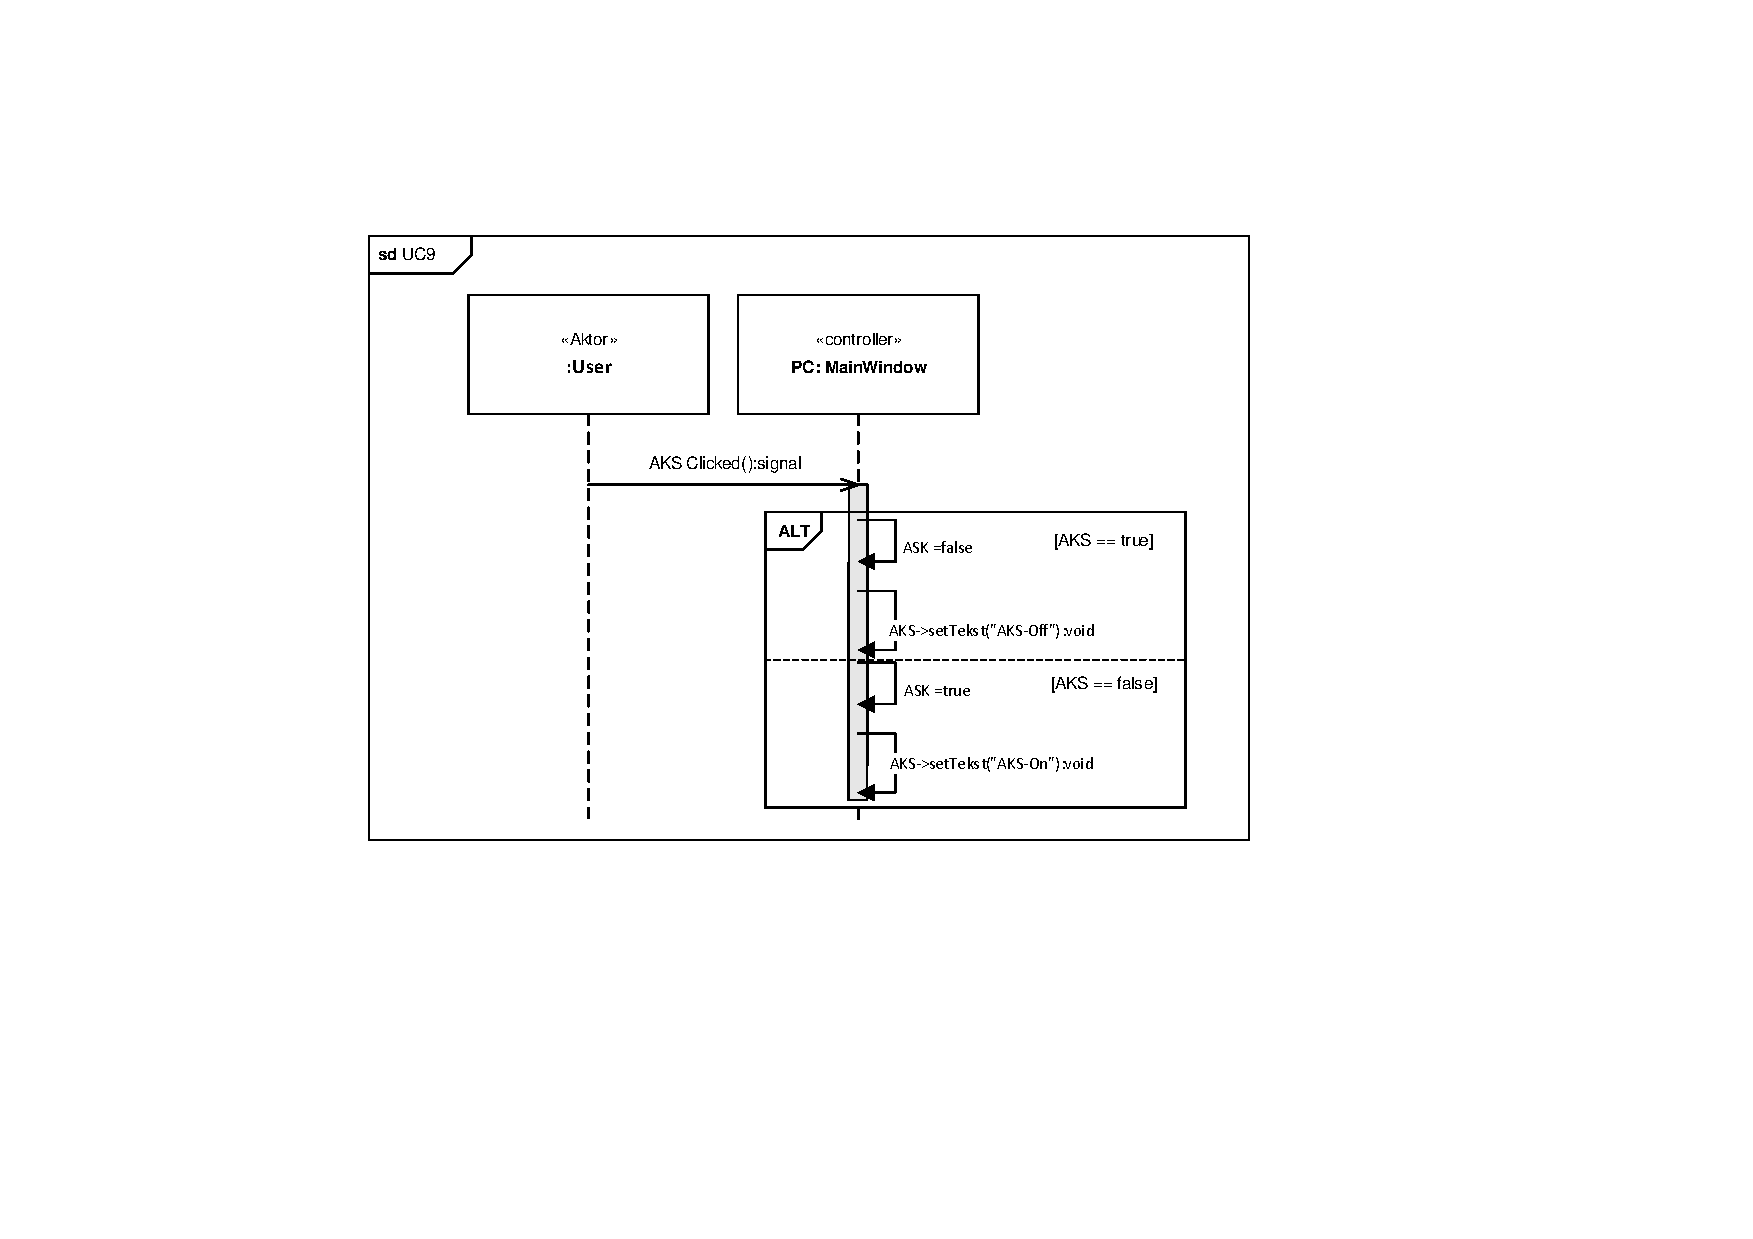
\includegraphics[width=\textwidth* 2/3,height=\textwidth* 4/10 ]{../fig/diagrammer/pc/sd_uc9.pdf}
\caption{Sekvensdiagram over UC9}
\label{fig:cd_uc9}
\end{figure}

\begin{figure}[H]
\centering
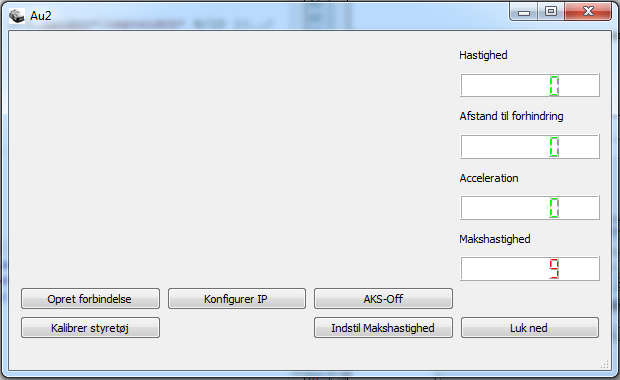
\includegraphics[width=\textwidth* 3/4,height=\textwidth* 9/20 ]{../fig/billeder/gui_uc9.png}
\caption{GUI UC9}
\label{fig:GUI_uc9}
\end{figure}

\clearpage

\subsubsection{UC10: Indstil makshastighed}
For at aktivere usecase 10 klikker bruger på \texttt{''Indstil makshastighed''}.
\texttt{MainWindow} åbner en inputdialog hvor i bruger indtaster et tal mellem 0 og 10. Inputdialogen accepterer ikke indtastninger uden for dette interval. Se sekvensdiagrammet i figur \ref{fig:cd_uc10} og indputdialogen i figur \ref{fig:GUI_uc10}

\begin{figure}[H]
\centering
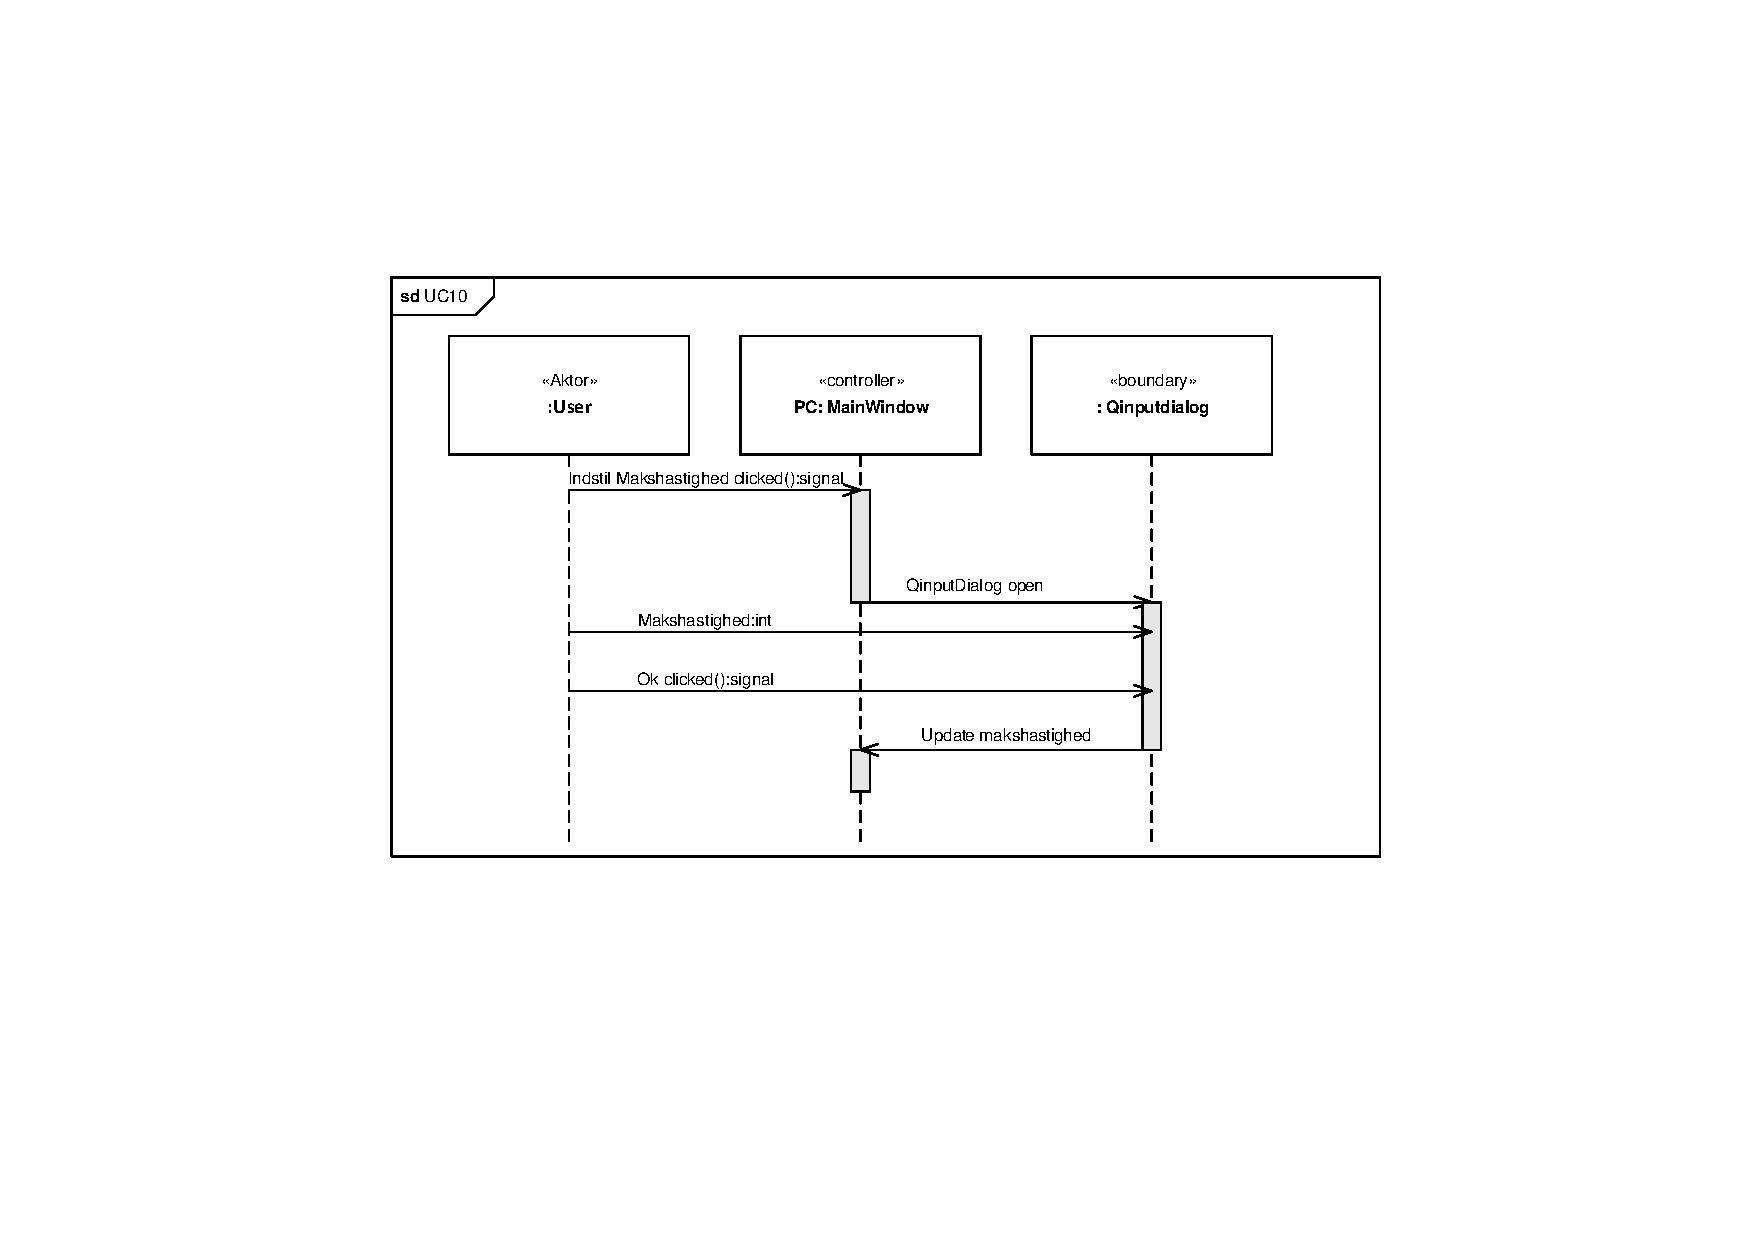
\includegraphics[width=\textwidth* 2/3,height=\textwidth* 4/10 ]{../fig/diagrammer/pc/sd_uc10.pdf}
\caption{Sekvensdiagram over UC10}
\label{fig:cd_uc10}
\end{figure}

\begin{figure}[H]
\centering
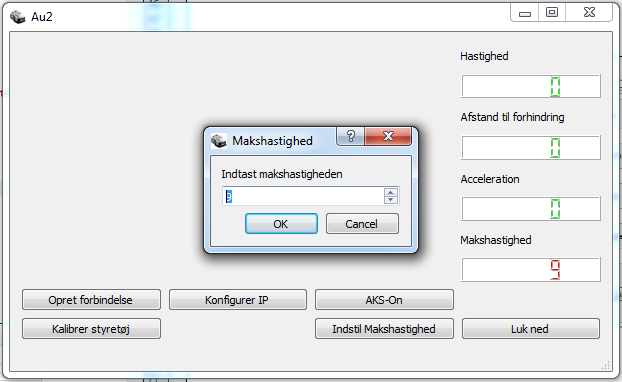
\includegraphics[width=\textwidth* 3/4,height=\textwidth* 9/20 ]{../fig/billeder/gui_uc10.png}
\caption{GUI UC10}
\label{fig:GUI_uc10}
\end{figure}

\clearpage

\subsubsection{UC11: Kalibrer styretøj}
For at aktivere usecase 11 klikker bruger på \texttt{''Kalibrer styretøj''}.
\texttt{MainWindow} åbner en inputdialog hvor i bruger indtaster et tal mellem -50 og 50. Inputdialogen accepterer ikke indtastninger uden for dette interval. Se sekvensdiagrammet i figur \ref{fig:cd_uc11} og indputdialogen i figur \ref{fig:GUI_uc11}

\begin{figure}[H]
\centering
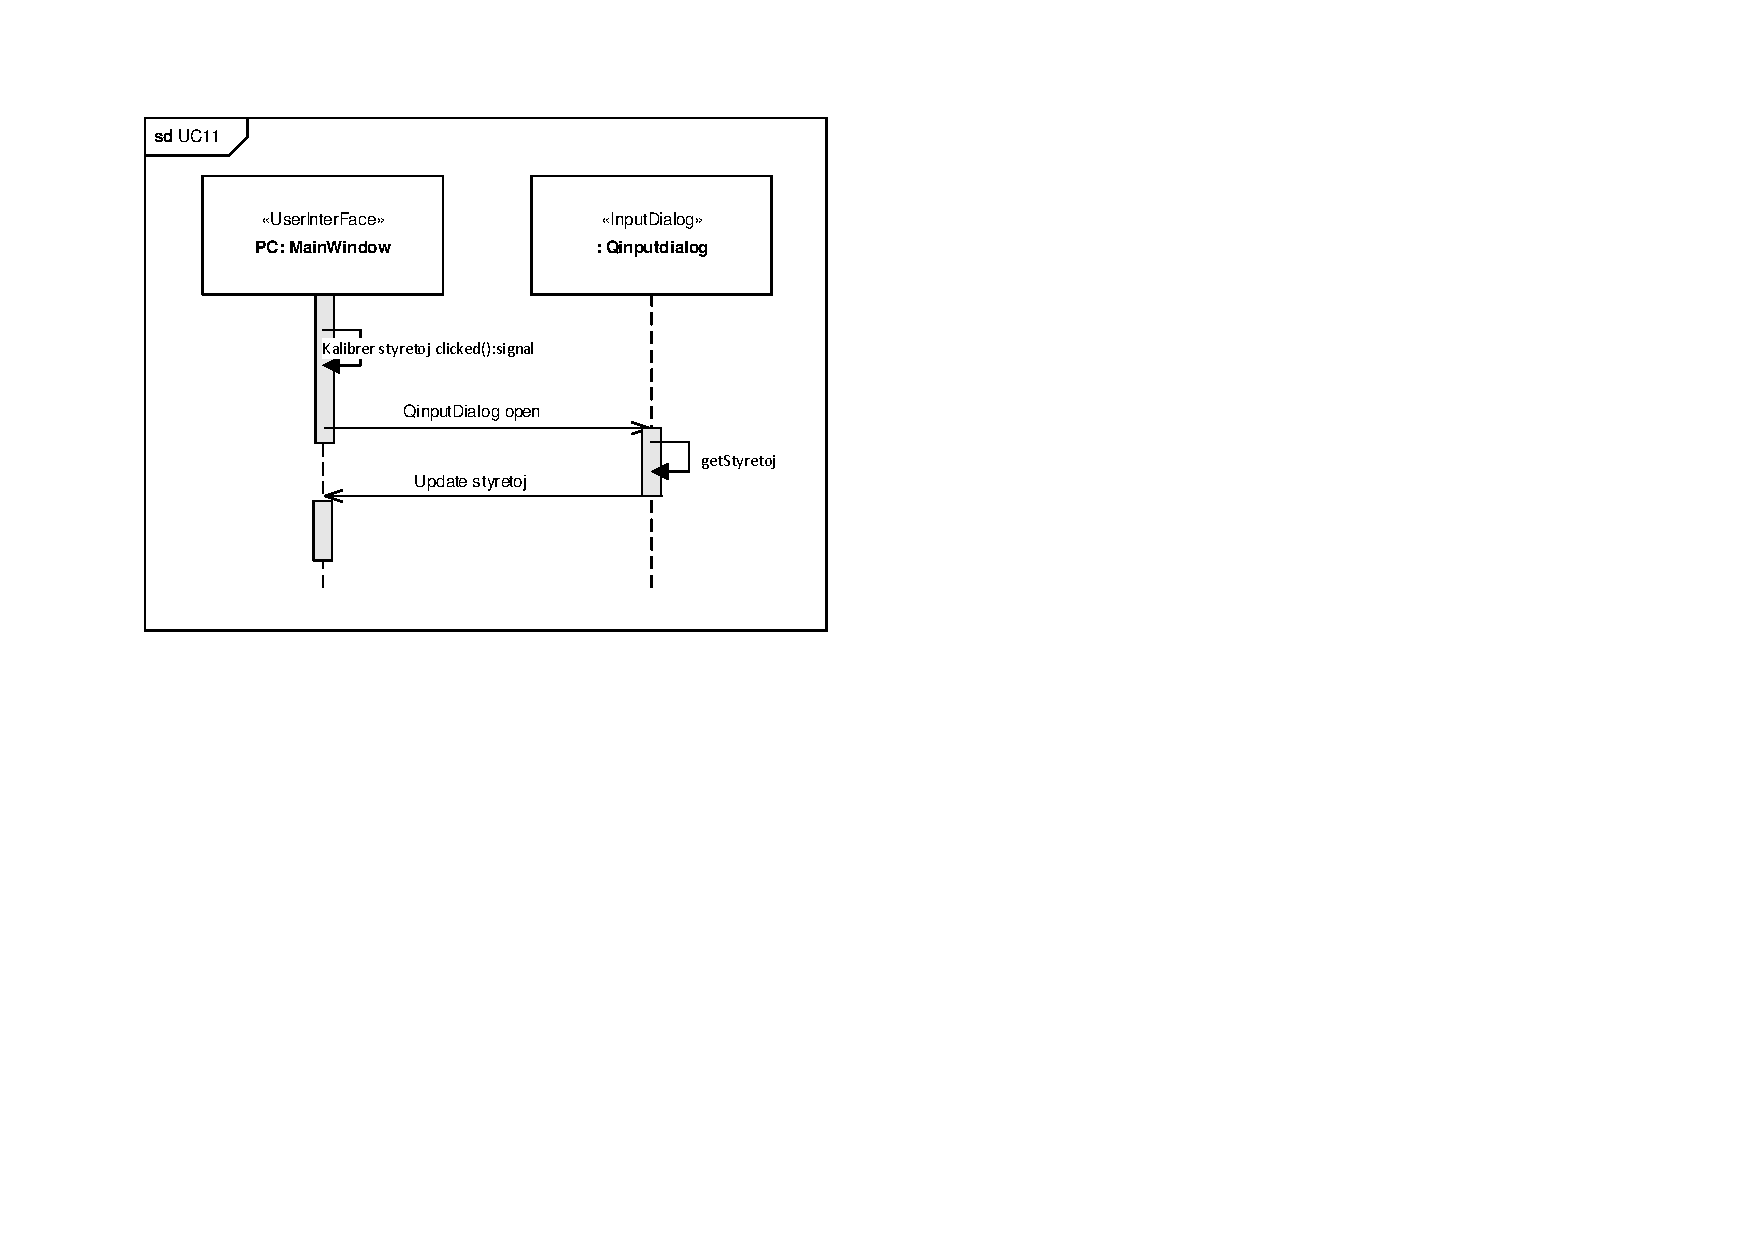
\includegraphics[width=\textwidth* 2/3,height=\textwidth* 4/10 ]{../fig/diagrammer/pc/sd_uc11.pdf}
\caption{Sekvensdiagram over UC11}
\label{fig:cd_uc11}
\end{figure}

\begin{figure}[H]
\centering
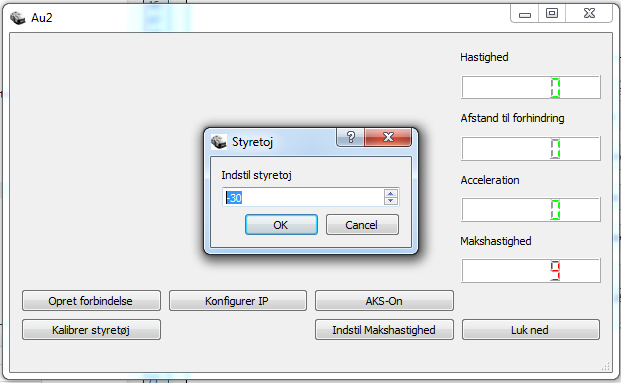
\includegraphics[width=\textwidth* 3/4,height=\textwidth* 9/20 ]{../fig/billeder/gui_uc11.png}
\caption{GUI UC11}
\label{fig:GUI_uc11}
\end{figure}

\clearpage

\subsubsection{UC12: Afbryd system}
For at aktivere usecase 11 klikker bruger på \texttt{''Luk ned''}.
\texttt{dataSocket} beder bilen om at lukke ned og bilen svarer med et ACK. Modtages der ikke et ACK giver \texttt{MainWindow} bruger besked om at bilen ikke kan lukke ned. Se sekvensdiagrammet i figur \ref{fig:cd_uc11} og advarslen i figur \ref{fig:GUI_uc11}

\begin{figure}[H]
\centering
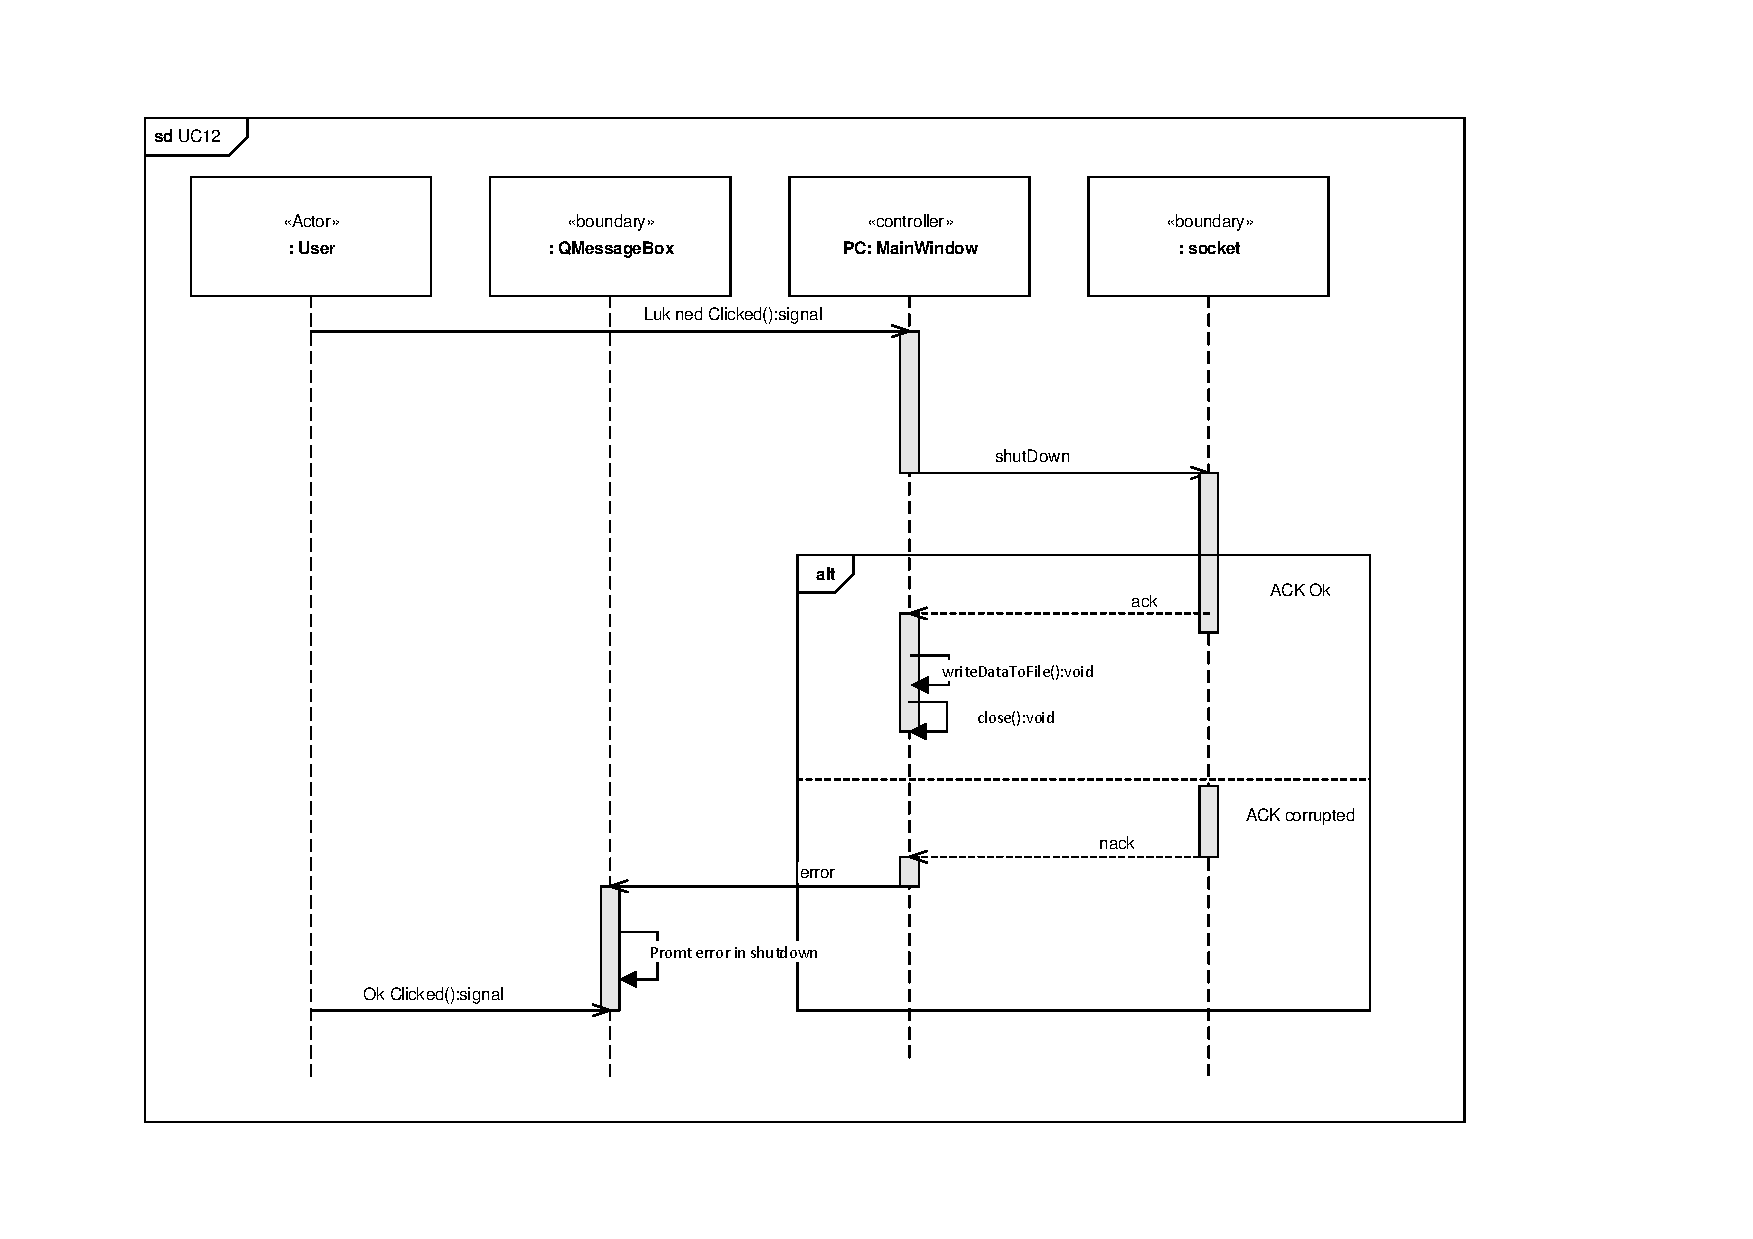
\includegraphics[width=\textwidth* 2/3,height=\textwidth* 4/10 ]{../fig/diagrammer/pc/sd_uc12.pdf}
\caption{Sekvensdiagram over UC12}
\label{fig:cd_uc12}
\end{figure}

\begin{figure}[H]
\centering
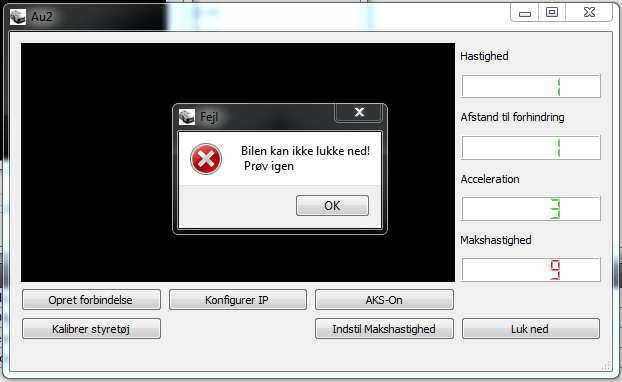
\includegraphics[width=\textwidth* 3/4,height=\textwidth* 9/20 ]{../fig/billeder/gui_uc12.png}
\caption{GUI UC12}
\label{fig:GUI_uc12}
\end{figure}

\clearpage

\subsection{Klassebeskrivelse}
I denne sektion vil der blive beskrevet klassen \texttt{MainWindow}. \texttt{MainWindow} er GUI'ens hoved klasse hvor i alt styres fra. \texttt{XboxController} er controllerens klasse som \texttt{MainWindow} bruger til at streame controllerdata fra.

\begin{figure}[H]
\centering
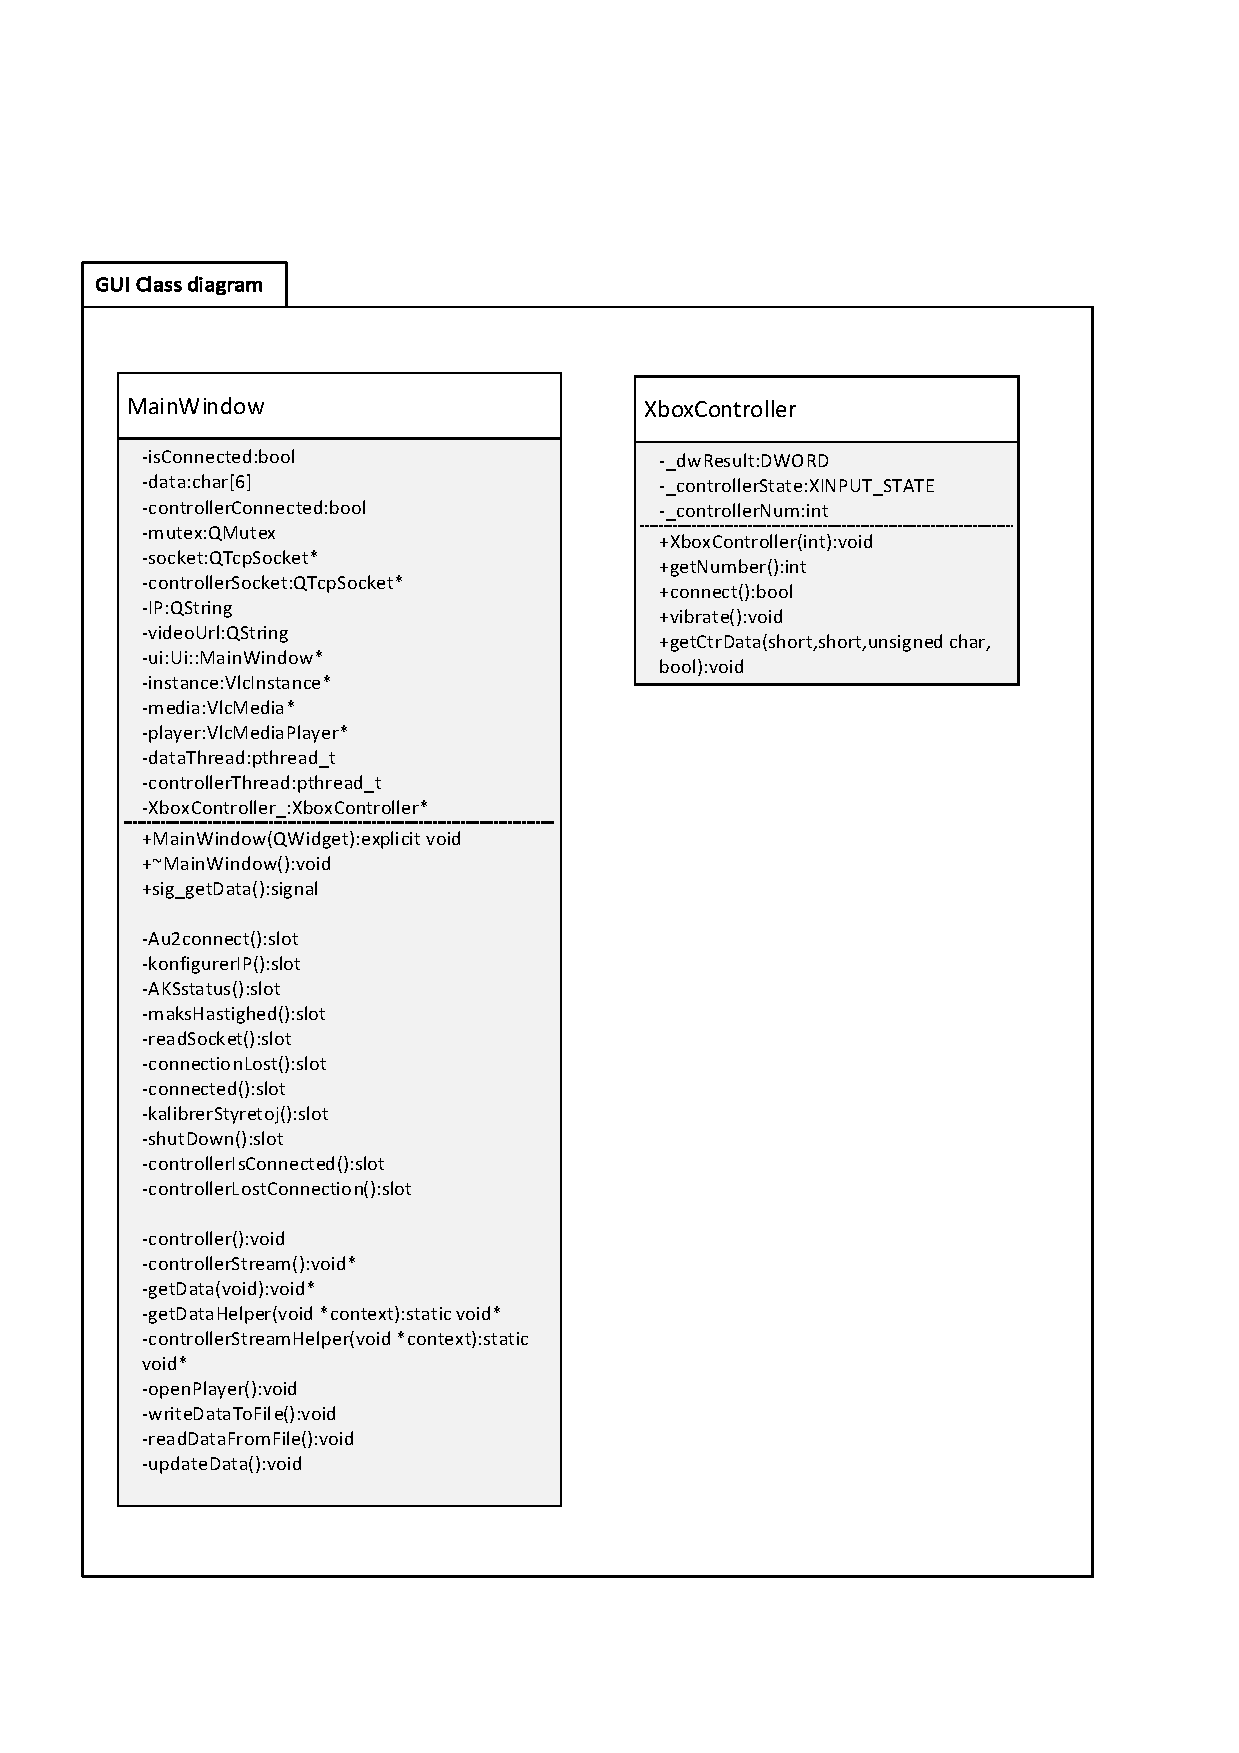
\includegraphics[width=\textwidth* 9/10]{../fig/diagrammer/pc/gui_classdiagram.pdf}
\caption{Klasse diagram over GUI}
\label{fig:cd_gui}
\end{figure}
\clearpage
\textbf{Attributter for MainWindow}

\begin{table}[H]
\begin{tabularx}{\textwidth}{| L{2.5cm} | l | Z |} \hline
Navn & Type & Beskrivelse \\\hline
\texttt{isConnected}         & \texttt{bool}           &Bliver brugt til at angive om socket har forbindelse til bilen eller ej \\\hline
\texttt{data}                & \texttt{char[6]}        &Char array som indeholder: Hastighed, Makshastighed, AKS-status, Styretøj, Acceleration og Afstand\\\hline
\texttt{controller -Connected} & \texttt{bool}           &Bruges til at angive om Xbox360-controlleren er forbundet eller ej\\\hline
\texttt{mutex}               & \texttt{QMutex*}        &Bruges til at låse således data kun kan tilgås af en tråd af gangen\\\hline
\texttt{socket}              & \texttt{QTcpSocket*}    &Er selve datasocket instancen\\\hline
\texttt{controller -Socket}    & \texttt{QTcpSocket*}    &Er selve controllerSocket instansen\\\hline
\texttt{IP}                  & \texttt{QString}        &Indeholder IP-adressen på bilen\\\hline
\texttt{videoURL}            & \texttt{QString}        &Indeholder adressen på videostreamet fra bilen\\\hline
\texttt{ui::Ui}              & \texttt{MainWindow*}    &Selve GUI'en\\\hline
\texttt{instance}            & \texttt{VlcInstance*}   &Bruges til at afspille videostream\\\hline
\texttt{media}               & \texttt{VlcMedia*}      &Bruges til at afspille videostream\\\hline
\texttt{player}              & \texttt{VlcMediaPlay -er*}&Bruges til at afspille videostream\\\hline
\texttt{dataThread}          & \texttt{p\_thread\_t}     &Er selve data tråden\\\hline
\texttt{controller -Thread}    & \texttt{p\_thread\_t}     &Er selve controller tråden\\\hline
\texttt{XboxControl -ler\_}     & \texttt{XboxControl -ler*}&En instance af Xbox360-controlleren\\\hline
\texttt{sig\_getData}     & \texttt{signal}&dataThread bruger dette signal til at give besked til MainWindow om at køre funktionen readSocket \\\hline

\end{tabularx}
\caption{Attributter for klassen MainWindow}
\label{table:attr_distancesensor}
\end{table}

\textbf{Metoder for MainWindow}

\begin{table}[H]
\begin{tabularx}{\textwidth}{| l | Z |} \hline
Prototype & \texttt{explicit void MainWindow()} \\\hline
Parametre &  QWidget \\\hline
Returværdi &  \\\hline
Beskrivelse & Er \texttt{MainWindows} constructor. Bruges til at indlæse data fra logfilen så bruger kan se gamle indtastede værdier, samt opdatere hovedvinduet, forbinde \texttt{signals and slots}, initiere variabler til deres default værdi og oprette en instans af VLC player. Playeren åbnes dog først når en socketforbindelse er oprettet.   \\\hline
\end{tabularx}
\caption{Metodebeskrivelse for \texttt{MainWindow}}
\label{table:met_MainWindow}
\end{table}


\clearpage

\begin{table}[H]
\begin{tabularx}{\textwidth}{| l | Z |} \hline
Prototype & \texttt{void $\sim$MainWindow()} \\\hline
Parametre &  \\\hline
Returværdi &  \\\hline
Beskrivelse & Er \texttt{MainWindows} destructor. Bruges til at slette oprettede instanser. \\\hline
\end{tabularx}
\caption{Metodebeskrivelse for \texttt{$\sim$MainWindow}}
\label{table:met_sMainWindow}
\end{table}


\begin{table}[H]
\begin{tabularx}{\textwidth}{| l | Z |} \hline
Prototype & \texttt{slot void Au2connect()} \\\hline
Parametre &   \\\hline
Returværdi &  \\\hline
Beskrivelse & Kaldes når bruger trykker på \texttt{''Opret forbindelse''}. Bruges til at skabe forbindelse mellem bil og Pc samt oprette \texttt{dataThread} og \texttt{Xbox360ControllerThread} samt forbinde \texttt{signals and slots}. Når der ikke kan oprettes forbindelse skabes der et advarselsvindue hvori der gives besked til brugeren om at forbindelsen ikke kunne skabes. Oprettes forbindelsen oprettes der samtidig et meddelelsesvindue hvor brugeren gives besked herom. Er forbindelsen oprettet sørger denne funktion også for at åbne VLC-playeren i hovedvinduet. \\\hline
\end{tabularx}
\caption{Metodebeskrivelse for \texttt{Au2connect}}
\label{table:met_Au2connect}
\end{table}

\begin{table}[H]
\begin{tabularx}{\textwidth}{| l | Z |} \hline
Prototype & \texttt{slot void konfigurerIp()} \\\hline
Parametre &   \\\hline
Returværdi &  \\\hline
Beskrivelse & Kaldes når bruger trykker på \texttt{''Konfigurer IP''}. Bruges til at opdatere variablen \texttt{IP} med brugerinput. En inputdialog åbnes hvor brugeren indtaster en IP-adresse. IP-adressen gemmes i variablen \texttt{IP}. Variablen \texttt{videoURL} sættes til "http://"+IP+":8081/stream.mjpeg" \\\hline
\end{tabularx}
\caption{Metodebeskrivelse for \texttt{konfigurerIp}}
\label{table:met_konfigurerIp}
\end{table}

\begin{table}[H]
\begin{tabularx}{\textwidth}{| l | Z |} \hline
Prototype & \texttt{slot void AKSstatus()} \\\hline
Parametre &   \\\hline
Returværdi &  \\\hline
Beskrivelse & Kaldes når bruger klikker på \texttt{''AKS-On''} eller \texttt{''AKS-Off''}. Bruges til at ændre status på AKS. \texttt{data[4]} sættes til henholdsvis 1 eller 0. Teksten på knappen ændres enten til \texttt{''AKS-Off''} eller \texttt{''AKS-On''} afhængig af en nuværende værdi af AKS. \\\hline
\end{tabularx}
\caption{Metodebeskrivelse for \texttt{AKSstatus}}
\label{table:met_AKSstatus}
\end{table}

\clearpage
\begin{table}[H]
\begin{tabularx}{\textwidth}{| l | Z |} \hline
Prototype & \texttt{slot void maksHastighed} \\\hline
Parametre &   \\\hline
Returværdi &  \\\hline
Beskrivelse & Kaldes når bruger klikker på \texttt{''Indstil makshastighed''}. Bruges til at ændre makshastigheden på bilen. En inputdialog åbnes hvori bruger kan indtaste en værdi mellem 0 og 10. Inputdialogen blokere selv for indtastninger uden for dette interval.  \\\hline
\end{tabularx}
\caption{Metodebeskrivelse for \texttt{maksHastighed}}
\label{table:met_maksHastighed}
\end{table}

\begin{table}[H]
\begin{tabularx}{\textwidth}{| l | Z |} \hline
Prototype & \texttt{slot void readSocket()} \\\hline
Parametre &   \\\hline
Returværdi &  \\\hline
Beskrivelse & \texttt{dataThread} giver signalet \texttt{sig\_getData} som modtages af \texttt{MainWindow} der herved eksekverer denne funktion. I funktionen låses \texttt{mutex} så \texttt{MainWindow} ikke kan tilgå data arrayet samtidig. Data arrayet sendes til bilen, derefter sender bilen dens data som igen modtages i data arrayet. Efter modtagelse af data oplåses \texttt{mutex}. \\\hline
\end{tabularx}
\caption{Metodebeskrivelse for \texttt{readSocket}}
\label{table:met_readSocket}
\end{table}

\begin{table}[H]
\begin{tabularx}{\textwidth}{| l | Z |} \hline
Prototype & \texttt{slot void connectionLost()} \\\hline
Parametre &   \\\hline
Returværdi &  \\\hline
Beskrivelse & Når \texttt{dataSocket} mister forbindelse gives signalet \texttt{disconnected} som er forbundet til denne funktion. Det vil sige at denne funktion køres når forbindelsen er mistet. Funktionen sætter variablen \texttt{isConnected} til \textbf{false}  \\\hline
\end{tabularx}
\caption{Metodebeskrivelse for \texttt{connectionLost}}
\label{table:met_connectionLost}
\end{table}

\begin{table}[H]
\begin{tabularx}{\textwidth}{| l | Z |} \hline
Prototype & \texttt{slot void connected()} \\\hline
Parametre &   \\\hline
Returværdi &  \\\hline
Beskrivelse & Når \texttt{dataSocket} har oprettet forbindelse gives signalet \texttt{connected} som er forbundet til denne funktion. Det vil sige at denne funktion køres når forbindelsen er oprettet. Funktionen sætter variablen \texttt{isConnected} til \textbf{true}  \\\hline
\end{tabularx}
\caption{Metodebeskrivelse for \texttt{connected}}
\label{table:met_connected}
\end{table}


\begin{table}[H]
\begin{tabularx}{\textwidth}{| l | Z |} \hline
Prototype & \texttt{slot void kalibrerStyretoj()} \\\hline
Parametre &   \\\hline
Returværdi &  \\\hline
Beskrivelse & Kaldes når bruger klikker på \texttt{''Kalibrer styretøj''}. Bruges til at kalibrere styretøjet på bilen. En inputdialog åbnes hvor det er mulig for brugeren at indtaste en værdi mellem -50 og 50. Inputdialogen blokerer selv for input udover dette interval. \texttt{data[5]} opdateres med værdien. \\\hline
\end{tabularx}
\caption{Metodebeskrivelse for \texttt{kalibrerStyretoj}}
\label{table:met_kalibrerStyretoj}
\end{table}

\begin{table}[H]
\begin{tabularx}{\textwidth}{| l | Z |} \hline
Prototype & \texttt{slot void shutDown()} \\\hline
Parametre &   \\\hline
Returværdi &  \\\hline
Beskrivelse & Kaldes når bruger klikker på \texttt{''Luk ned''} eller klikker i det røde kryds i hovedvinduet. Sørger for at sende besked til bilen om at lukke dens software sikkert ned. Når funktionen køres tester den om \texttt{isConnected} er true, hvis den er skrives der \textbf{"dwnnow"} til bilen. Retuneres \textbf{"dwnnow"} fra bilen bliver \texttt{dataSocket} disconnected og \texttt{destructoren} kaldes. Modtages der andet en \textbf{"dwnnow"} fra bilen skabes der et advarselsvindue til brugeren om at bilen ikke kan lukke sikkert ned. \\\hline
\end{tabularx}
\caption{Metodebeskrivelse for \texttt{shutDown}}
\label{table:met_shutDown}
\end{table}

\begin{table}[H]
\begin{tabularx}{\textwidth}{| l | Z |} \hline
Prototype & \texttt{slot void controllerIsConnected()} \\\hline
Parametre &   \\\hline
Returværdi &  \\\hline
Beskrivelse & Eksekveres når controlleren er forbundet til bilen. \texttt{controllerSocket} giver signalet \texttt{connected} som er forbundet til denne funktion. Funktionen sætter variablen \texttt{controllerConnected} til \textbf{true}.   \\\hline
\end{tabularx}
\caption{Metodebeskrivelse for \texttt{controllerIsConnected}}
\label{table:met_controllerIsConnected}
\end{table}

\begin{table}[H]
\begin{tabularx}{\textwidth}{| l | Z |} \hline
Prototype & \texttt{slot void controllerLostConnection()} \\\hline
Parametre &   \\\hline
Returværdi &  \\\hline
Beskrivelse & Eksekveres når controlleren mister forbundet til bilen. \texttt{controllerSocket} giver signalet \texttt{disconnected} som er forbundet til denne funktion. Funktionen sætter variablen \texttt{controllerConnected} til \textbf{false}.   \\\hline
\end{tabularx}
\caption{Metodebeskrivelse for \texttt{controllerLostConnection}}
\label{table:met_ccontrollerLostConnection}
\end{table}

\begin{table}[H]
\begin{tabularx}{\textwidth}{| l | Z |} \hline
Prototype & \texttt{void controller()} \\\hline
Parametre &   \\\hline
Returværdi &  \\\hline
Beskrivelse & Kaldes af \texttt{Au2Connect} når \texttt{dataSocket} er forbundet. Funktionen opretter en ny instance af \texttt{XboxController} og tester efterfølgende om controlleren er forbundet. Er controlleren ikke forbundet oprettes en advarselsmeddelelse hvor bruger gives besked herom. Er controlleren forbundet oprettes der en ny instance af \texttt{controllerSocket} og \texttt{signals and slots} forbindes. \texttt{controllerSocket} forbindes til bilen. Kan der ikke skabes forbindelse oprettes der en advarselsmeddelelse hvor bruger gives besked herom. Skabes forbindelsen retunerer funktionen herefter.  \\\hline
\end{tabularx}
\caption{Metodebeskrivelse for \texttt{controller}}
\label{table:met_controller}
\end{table}

\clearpage

\begin{table}[H]
\begin{tabularx}{\textwidth}{| l | Z |} \hline
Prototype & \texttt{void* controllerStream()} \\\hline
Parametre &   \\\hline
Returværdi &  \\\hline
Beskrivelse & Funktionen kører i en while-løkke sålænge variablen \texttt{controllerConnected} er \textbf{true}. I while-løkken hentes data fra controlleren som efterfølgende sendes til bilen igennem \texttt{controllerSocket}. Herefter ventes 10ms før sekvensen gentages. Funktionen køres af \texttt{controllerThread}.\\\hline
\end{tabularx}
\caption{Metodebeskrivelse for \texttt{controllerStream}}
\label{table:met_controllerStream}
\end{table}

\begin{table}[H]
\begin{tabularx}{\textwidth}{| l | Z |} \hline
Prototype & \texttt{static void* controllerStreamHelper()} \\\hline
Parametre & void* context  \\\hline
Returværdi & Funktionspointer tilcontrollerStream  \\\hline
Beskrivelse & Kaldes af \texttt{pthread\_create} og retunerer funktionspointeren til \texttt{controllerStream}. Dette gøres fordi pthread kun kan tilgå \texttt{static} funktioner og at \texttt{static} funktioner kun kan tilgå \texttt{static} variabler. Dette giver et problem da \texttt{controllerStream} ikke tilgår \texttt{static} variabler og derfor ikke kan gøres \texttt{static}. \texttt{pthread\_create} eksekverer således \texttt{controllerstream} som \texttt{controllerThread}.\\\hline
\end{tabularx}
\caption{Metodebeskrivelse for \texttt{controllerStreamHelper}}
\label{table:met_controllerStreamHelper}
\end{table}

\begin{table}[H]
\begin{tabularx}{\textwidth}{| l | Z |} \hline
Prototype & \texttt{void* getData()} \\\hline
Parametre &   \\\hline
Returværdi &  \\\hline
Beskrivelse & Funktionen kører i en while-løkke sålænge variablen \texttt{isConnected} er \textbf{true}. I while-løkken gives signalet \texttt{sig\_getData} som gør at \texttt{MainWindow} eksekverer funktionen \texttt{readSocket} og herved opdaterer data arrayet. Efter signalet er givet kaldes funktionen \texttt{updateData} som opdaterer hovedvinduet. Herefter ventes 100ms før sekvensen gentages.  \\\hline
\end{tabularx}
\caption{Metodebeskrivelse for \texttt{getData}}
\label{table:met_getData}
\end{table}

\begin{table}[H]
\begin{tabularx}{\textwidth}{| l | Z |} \hline
Prototype & \texttt{static void* getDataHelper()} \\\hline
Parametre & void* context  \\\hline
Returværdi & Funktionspointer getData  \\\hline
Beskrivelse & Kaldes af \texttt{pthread\_create} og retunerer funktionspointeren til \texttt{getData}. Dette gøres fordi pthread kun kan tilgå \texttt{static} funktioner og at \texttt{static} funktioner kun kan tilgå \texttt{static} variabler. Dette giver et problem da \texttt{getData} ikke tilgår \texttt{static} variabler og derfor ikke kan gøres \texttt{static}. \texttt{pthread\_create} eksekverer således \texttt{getData} som dataThread.\\\hline
\end{tabularx}
\caption{Metodebeskrivelse for \texttt{getDataHelper}}
\label{table:met_getDataHelper}
\end{table}

\clearpage

\begin{table}[H]
\begin{tabularx}{\textwidth}{| l | Z |} \hline
Prototype & \texttt{void openPlayer()} \\\hline
Parametre &  \\\hline
Returværdi &  \\\hline
Beskrivelse & Åbner instansen af VLC-player i hovedvinduet. Kaldes når \texttt{dataSocket} er forbundet.  \\\hline
\end{tabularx}
\caption{Metodebeskrivelse for \texttt{openPlayer}}
\label{table:met_openPlayer}
\end{table}

\begin{table}[H]
\begin{tabularx}{\textwidth}{| l | Z |} \hline
Prototype & \texttt{void writeDataToFile()} \\\hline
Parametre &  \\\hline
Returværdi &  \\\hline
Beskrivelse & Skriver data-arrayet til log filen når GUI'en lukkes ned. Filen \texttt{AutoData.txt} belliggende i samme folder som \texttt{Au2.exe}, åbnes og indholdet af data arrayet skrives ud.  \\\hline
\end{tabularx}
\caption{Metodebeskrivelse for \texttt{writeDataToFile}}
\label{table:met_writeDataToFile}
\end{table}

\begin{table}[H]
\begin{tabularx}{\textwidth}{| l | Z |} \hline
Prototype & \texttt{void readDataFromFile()} \\\hline
Parametre &  \\\hline
Returværdi &  \\\hline
Beskrivelse & Læser data-arrayet fra log filen når \texttt{contructoren} kaldes.  \\\hline
\end{tabularx}
\caption{Metodebeskrivelse for \texttt{readDataFromFile}}
\label{table:met_readDataFromFile}
\end{table}

\begin{table}[H]
\begin{tabularx}{\textwidth}{| l | Z |} \hline
Prototype & \texttt{void updateData()} \\\hline
Parametre &  \\\hline
Returværdi &  \\\hline
Beskrivelse & Opdatere hovedvinduet med data arrayet. \\\hline
\end{tabularx}
\caption{Metodebeskrivelse for \texttt{updateData}}
\label{table:met_updateData}
\end{table}

\clearpage
\subsubsection{Boundry-klasse: XboxController}

Denne klasse har til formål at agere API for Xbox Controlleren til PC softwaren. Til dette skal udnyttes standard biblioteket; XInput. Det skal være muligt at få alt det data der udnyttes til at bestemme bilens retning, ved et enkelt funktionskald for simplicitet. På Figur \ref{fig:cd_xboxcontroller} kan ses et klasse diagram over den ønskede klasse efterfulgt af funktionalitet.

\begin{figure}[h]
\centering
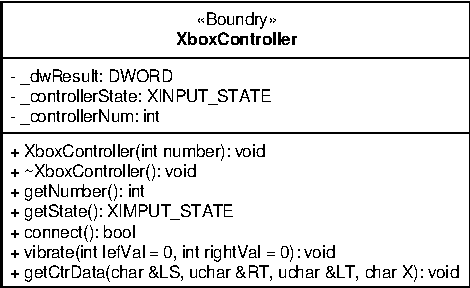
\includegraphics[]{../fig/diagrammer/pc/cd_xboxcontroller.pdf}
\caption{Klassebeskrivelse for boundry-klassen XboxController}
\label{fig:cd_xboxcontroller}
\end{figure}

\textbf{Attributter}

\begin{table}[h]
\begin{tabularx}{\textwidth}{| Z | Z | L{10cm} |} \hline
Navn & Type & Beskrivelse \\\hline
\texttt{\_dwResult}				& \texttt{DWORD}		&Variabel af typen DWORD, skal indeholde data om controllerens tilstand.\\\hline

\texttt{\_controller- State}	& \texttt{XINPUT\_STATE}&Struct af typen XINPUT\_STATE. Indeholder hhv. DWORD, der indeholder en værdi forskellig fra 0 hvis der er sket en ændring i controllerens tilstand, og XINPUT\_GAMEPAD, der indeholder alle værdier som fortæller om controllerens nuværende tilstand.\\\hline

\texttt{\_controller- Num}		& \texttt{int}			&Variabel af typen int der indeholder controller nummer.\\\hline
\end{tabularx}
\caption{Attributter for klassen XboxController}
\label{table:attr_xboxcontroller}
\end{table}

\textbf{Metoder}

\begin{table}[h]
\begin{tabularx}{\textwidth}{| L{2.5 cm} | Z |} \hline
Prototype 	& \texttt{void XboxController(int number)} \\\hline
Parametre 	& \texttt{number} 			\newline Det ønskede controller ID (1-4). \\\hline
Returværdi	& \texttt{void} 			\newline \\\hline
Beskrivelse	& Constructor til klassen XboxController. \newline \\\hline
\end{tabularx}
\caption{Metodebeskrivelse for constructoren af \texttt{XboxController} klassen}
\label{table:met_xboxcontroller}
\end{table}

\clearpage

\begin{table}[h]
\begin{tabularx}{\textwidth}{| L{2.5 cm} | Z |} \hline
Prototype 	& \texttt{void $\sim$XboxController()} \\\hline
Parametre 	& \texttt{void}				\newline \\\hline
Returværdi	& \texttt{void} 			\newline \\\hline
Beskrivelse	& Destructor til klassen XboxController. \newline \\\hline
\end{tabularx}
\caption{Metodebeskrivelse for destructoren af \texttt{XboxController} klassen}
\label{table:met_xboxcontroller_de}
\end{table}

\begin{table}[h]
\begin{tabularx}{\textwidth}{| L{2.5 cm} | Z |} \hline
Prototype 	& \texttt{int getNumber()} \\\hline
Parametre 	& \texttt{void}				\newline \\\hline
Returværdi	& \texttt{int} 				\newline Controllerens ID \\\hline
Beskrivelse	& Denne funktion har til formål at returnere objektets ID. \newline \\\hline
\end{tabularx}
\caption{Metodebeskrivelse for \texttt{getNumber()}}
\label{table:met_getnumber}
\end{table}

\begin{table}[h]
\begin{tabularx}{\textwidth}{| L{2.5 cm} | Z |} \hline
Prototype 	& \texttt{XINPUT\_STATE getState()} \\\hline
Parametre 	& \texttt{void}				\newline \\\hline
Returværdi	& \texttt{XINPUT\_STATE} 	\newline Struct af typen XINPUT\_STATE. Indeholder hhv. DWORD og XINPUT\_GAMEPAD. \\\hline
Beskrivelse	& Denne funktion har til formål at opdatere \_controllerState som indeholder controllerens nuværende tilstand og info om hvorvidt den har skiftet tilstand. \\\hline
\end{tabularx}
\caption{Metodebeskrivelse for \texttt{getState()}}
\label{table:met_getstate}
\end{table}

\begin{table}[h]
\begin{tabularx}{\textwidth}{| L{2.5 cm} | Z |} \hline
Prototype 	& \texttt{bool connect()} \\\hline
Parametre 	& \texttt{void}				\newline \\\hline
Returværdi	& \texttt{bool} 			\newline Controllerens connection tilstand \\\hline
Beskrivelse	&  Denne funktion returnerer hvorvidt der er forbindelse til controlleren. \\\hline
\end{tabularx}
\caption{Metodebeskrivelse for \texttt{connect()}}
\label{table:met_connect}
\end{table}

\clearpage

\begin{table}[h]
\begin{tabularx}{\textwidth}{| L{2.5 cm} | Z |} \hline
Prototype 	& \texttt{void vibrate(int leftVal = 0, int rightVal = 0)} \\\hline
Parametre 	& \texttt{leftVal}			\newline En værdi der fortæller controllerklassen hvor hurtigt vibrater motoren i venstre side af controlleren skal køre (0 - 65535).	\newline \newline
			  \texttt{rightVal}			\newline En værdi der fortæller controllerklassen hvor hurtigt vibrater motoren i højre side af controlleren skal køre (0 - 65535). \\\hline
Returværdi	& \texttt{void} 			\newline \\\hline
Beskrivelse	&  Denne funktion igangsætter højre og venstre vibrater med en styrke alt efter input parameterne leftVal og rightVal. Inputparameterne kan gå mellem 0 og 65535, hvor 0 er ingen vibrering og 65535 er maksimal vibrering. Hvis der ikke gives parametre med i funktionen, vil den automatisk sætte parameterne til 0 og dermed slukke for vibraterne.\\\hline
\end{tabularx}
\caption{Metodebeskrivelse for \texttt{vibrate()}}
\label{table:met_vibrate}
\end{table}

\begin{table}[h]
\begin{tabularx}{\textwidth}{| L{2.5 cm} | Z |} \hline
Prototype 	& \texttt{void getCtrlData(char \&LS, uchar \&RT, uchar \&LT, char X)} \\\hline
Parametre 	& \texttt{LS}				\newline En reference til den char der ønskes at funktionen indsætter data om controllerens ''Left Stick'' tilstand i.				\newline \newline
			  \texttt{RT}				\newline En reference til den unsigned char der ønskes at funktionen indsætter data om controllerens ''Right Trigger'' tilstand i.\newline \newline
			  \texttt{LT}				\newline En reference til den unsigned char der ønskes at funktionen indsætter data om controllerens ''Left Trigger'' tilstand i.\newline \newline
			  \texttt{X}				\newline En reference til den char der ønskes at funktionen indsætter data om controllerens ''X-button'' tilstand i. \\\hline
Returværdi	& \texttt{void} 			\newline \\\hline
Beskrivelse	&  Denne funktion har til formål at returnere nye controller tilstande, for controllerens Left Stick, Right Trigger, Left Trigger og X-button, på de refererede parametres plads.\\\hline
\end{tabularx}
\caption{Metodebeskrivelse for \texttt{getCtrlData()}}
\label{table:met_getctrldata}
\end{table}